\documentclass[tikz,border=8pt]{standalone}
% Shared look for every TikZ diagram. Load with \input{../../tools/tikz-style.tex}
\usepackage[T1]{fontenc}
\usepackage{lmodern}
\renewcommand{\sfdefault}{lmr}  % diagrams use the same serif as the text
\usetikzlibrary{arrows.meta, positioning, shapes.geometric, calc, fit, backgrounds}
\definecolor{cblue}{HTML}{4C78A8}
\definecolor{corange}{HTML}{F58518}
\definecolor{cgreen}{HTML}{54A24B}
\definecolor{cred}{HTML}{E45756}
\definecolor{cpurple}{HTML}{B279A2}
\definecolor{cgrey}{HTML}{6B6B6B}
\tikzset{
  every picture/.style={font=\sffamily, line width=1.2pt},
  box/.style={draw=#1, fill=#1!12, rounded corners=4pt, align=center, inner sep=7pt, minimum height=1.1cm},
  box/.default=cgrey,
  arrow/.style={-{Stealth[length=3mm]}, draw=cgrey, line width=1.4pt},
  title/.style={font=\sffamily\bfseries\Large},
  note/.style={font=\sffamily\small, text=cgrey, align=center},
}
\AtBeginDocument{\hyphenpenalty=10000 \exhyphenpenalty=10000}

\newcommand{\cell}[4]{\node[draw=cgrey, line width=0.8pt, minimum size=0.95cm, fill=#4, font=\sffamily\large] at ({#1},{#2}) {#3};}
\begin{document}
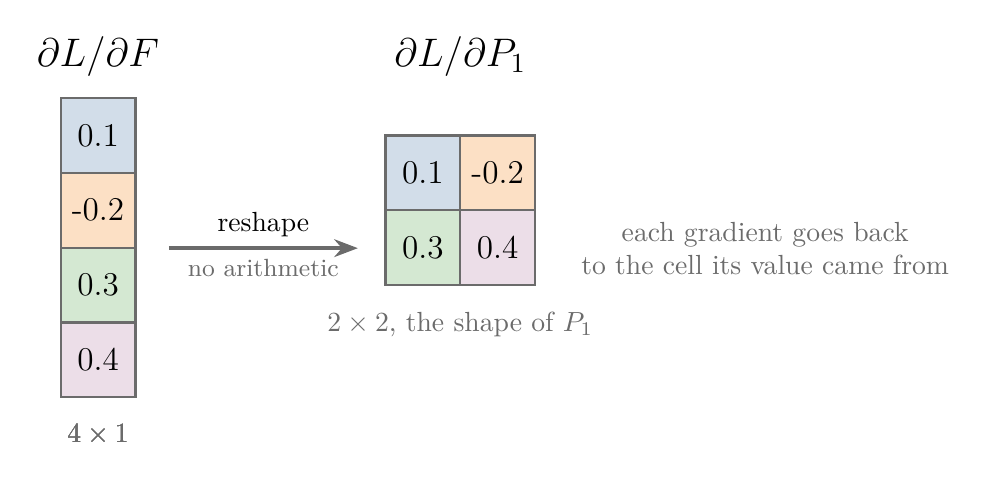
\begin{tikzpicture}
  \node[title] at (0,1.0) {$\partial L/\partial F$};
  \foreach \v/\c [count=\i from 0] in {0.1/cblue, -0.2/corange, 0.3/cgreen, 0.4/cpurple}
    \cell{0}{-\i*0.95}{\v}{\c!25}
  \node[note, font=\sffamily\normalsize] at (0,-3.8) {$4\times1$};
  \draw[arrow] (0.9,-1.43) -- (3.3,-1.43) node[midway, above] {reshape} node[midway, below, note] {no arithmetic};
  \node[title] at (4.6,1.0) {$\partial L/\partial P_1$};
  \foreach \v/\c [count=\i from 0] in {0.1/cblue, -0.2/corange, 0.3/cgreen, 0.4/cpurple}{
    \pgfmathtruncatemacro{\r}{\i/2}\pgfmathtruncatemacro{\cc}{mod(\i,2)}
    \cell{4.125+\cc*0.95}{-0.95-\r*0.95+0.475}{\v}{\c!25}
  }
  \node[note, font=\sffamily\normalsize] at (4.6,-2.4) {$2\times2$, the shape of $P_1$};
  \node[note, font=\sffamily\normalsize, anchor=west] at (6.0,-1.43) {each gradient goes back\\to the cell its value came from};
\end{tikzpicture}
\end{document}
